\documentclass[11pt]{article}
\usepackage{graphicx}
\graphicspath{{res/}}
\begin{document}
\title{Lec 13 \& 14 Notes \\ Classification Techniques}
\author{Hritik Soni \\ 2014A2PS0480P}
\date{}
\maketitle
\clearpage
\section{Introduction}
Classification is perhaps the most common type of problem encountered in all of machine learning.\\

In the process of classficiation, the learner has to identify the class of an object using existing training data and therefore this type of learning falls into the category of supervised learning. This is done by relating attributes of an object to its class which can be done in many ways and thus we have a bunch of techniques to do so. But we may not have the entire spectrum of training data so we may not reach 100\% accuracy but atleast we can try to do the best in our hands.
\section{Principle Component Analysis (PCA)}
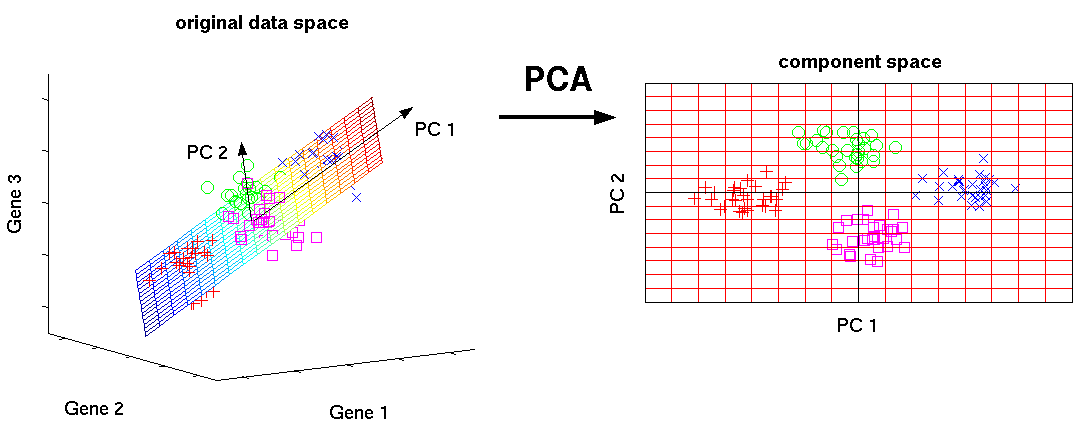
\includegraphics[width=\textwidth]{pca.png}
Often we deal with data containing a very high dimensionality. As the dimensionality of the data increases, so does the complexity of the model to be trained. This means higher training time as well as run time of our model. PCA is one of the most common techniques used to reduce the dimensionality of the data.\\

In this technique we try to project the given data in lower dimensions and try to see how much we are losing by looking at variances and so on. Often, it is observed that even after lowering dimensions by significant amounts we still retain the complete data information but we can stop after we lose lets say 0.1\% of the data.
\section{K-Nearest Neighbours Classifier (K-NN)}
The easiest approch to classify a unknown object would be to look for the most similar object in existing knowledge. There are a bunch of ways to calculate distance between two objects.\\

\noindent L1 or Manhattan Distance:\\

\noindent 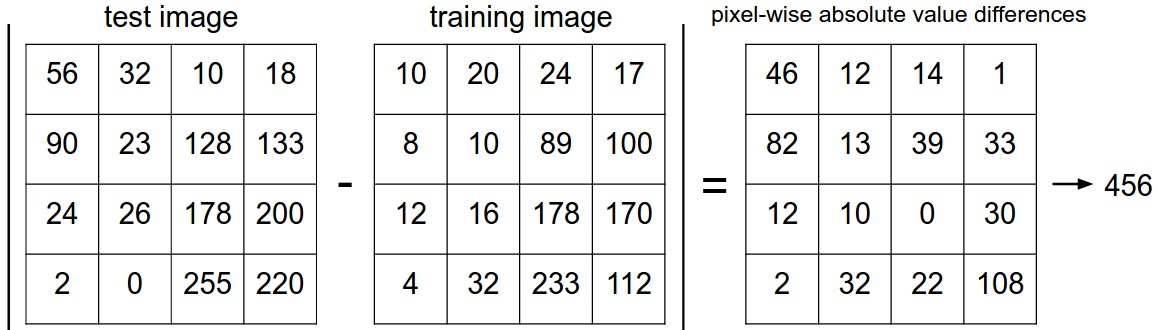
\includegraphics[width=\textwidth]{l1.jpeg}

\noindent We can also use L2 distance (Euclidein distance),

$$ d_{L2}(x, y) = \sqrt[2]{\sum_{i=1}^{n} (x_i - y_i)^2 }$$

Or, $L_p$

$$ d_{Lp}(x, y) = \sqrt[p]{\sum_{i=1}^{n} (x_i - y_i)^p }$$

Looking at a single sample can be misleading hence we find 'N' nearest neighbours and then take a vote to decide the label.\\

\noindent 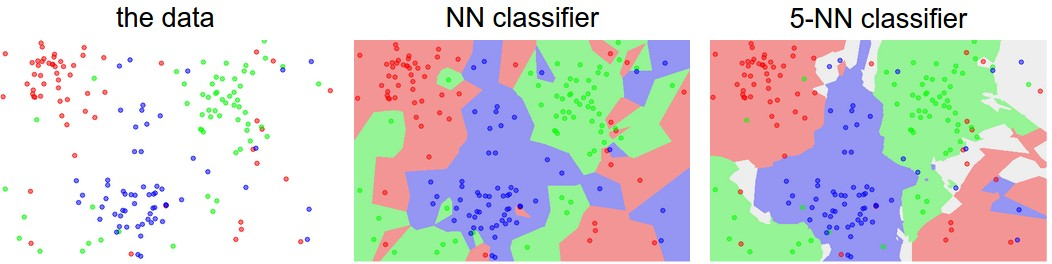
\includegraphics[width=\textwidth]{knn.jpeg}

\clearpage

\section{Linear Regression}

Linear regression is fitting a straight line or plane in higher dimensions.\\

\noindent 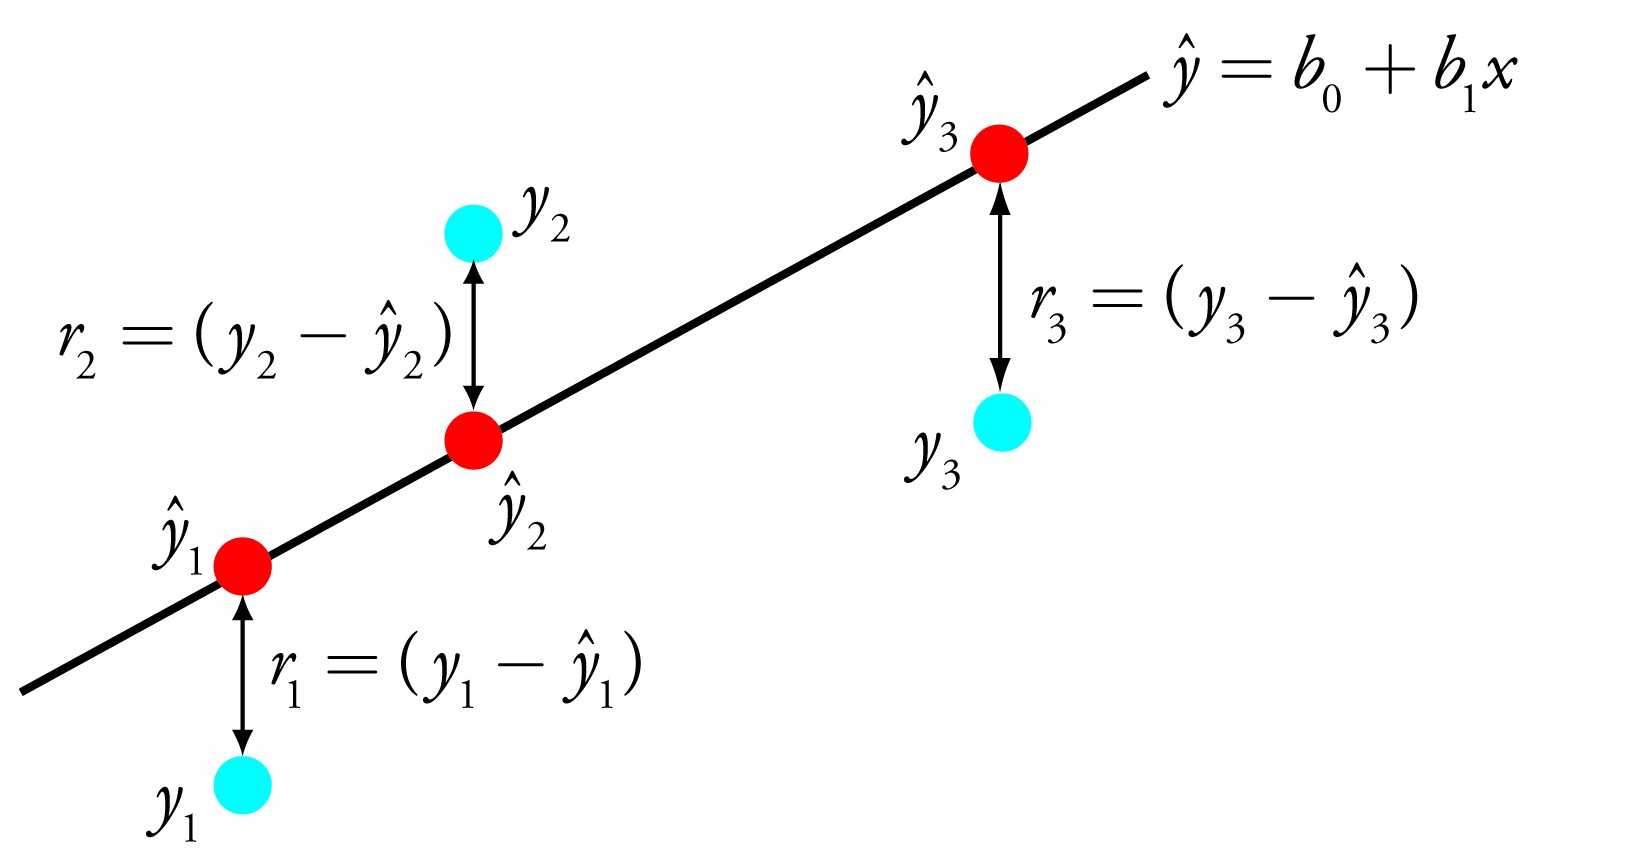
\includegraphics[width=\textwidth]{linear_reg.jpeg}
\noindent 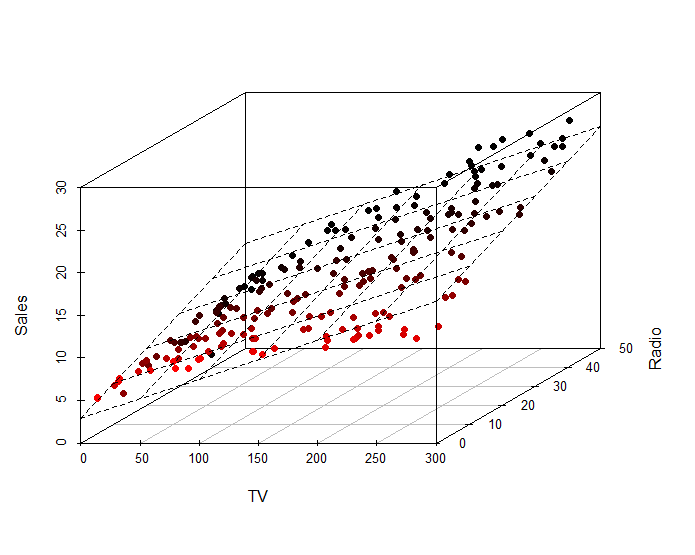
\includegraphics[width=\textwidth]{lr_3d.png}

\section{Decision Trees}

Decision Trees are supervised learning models used primarily for classification and sometimes for regression as well. The goal is to create a model that predicts the value of a target variable by learning simple decision rules inferred from the data features.\\

\noindent 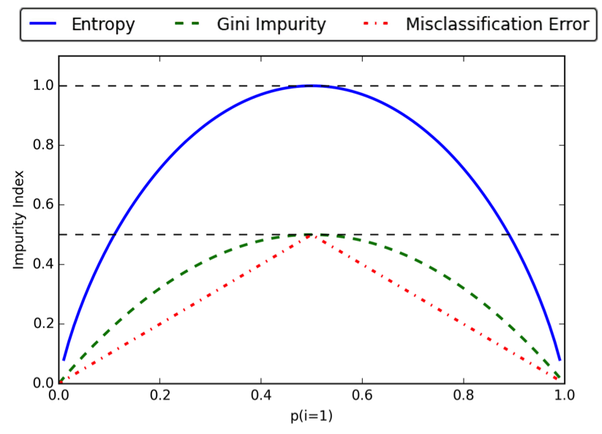
\includegraphics[width=\textwidth]{d-trees.png}

\clearpage

\section{Naive-Bayes Classifier}

Naive Bayes classifiers are a collection of classification algorithms based on Bayes’ Theorem. It is not a single algorithm but a family of algorithms where all of them share a common principle, i.e. every pair of features being classified is independent of each other.\\
With regards to our dataset, we can apply Bayes’ theorem in following way:\\
$$ P(y | X) = \frac{p(X | y) \cdot P(y)}{p(X)} $$
where, y is class variable and X is a dependent feature vector (of size n) where:
$$ X = (x_{1}, x_{2}, x_{3},....., x_{n}) $$

\clearpage

\section{Support Vector Machines (SVM)}

SVMs are another class of Classifiers that depend on features called Support Vectors. The following figure illustrates the working of SVMs\\

\noindent 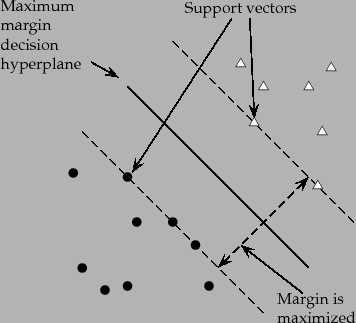
\includegraphics[width=\textwidth]{svm.png}

As can be observed in the picture, SVMs are linear classifiers that try to form a Maximum margin hyperplane such that margin between Support Vectors is maximized.

Support Vectors are points that can be used to form the maximum margin such that the resulting hyperplane separates the classes.

One of the most important benefits of SVM classification is that the hyperplane depends solely on the Support Vectors and not on the remaining points in the dataset. This means that a change in the non support vector points in the datset won't affect our model as opposed to other classifiers. Also, SVMs are not affected by outliers.

\section{Neural Networks or Multi-Layer Perceptron (MLP)}

Neural Networks are modelled to mimic the neurons present in human body. It is one of the most prominent nature inspired machine learning models. A typical neuron looks like the following:\\

\noindent 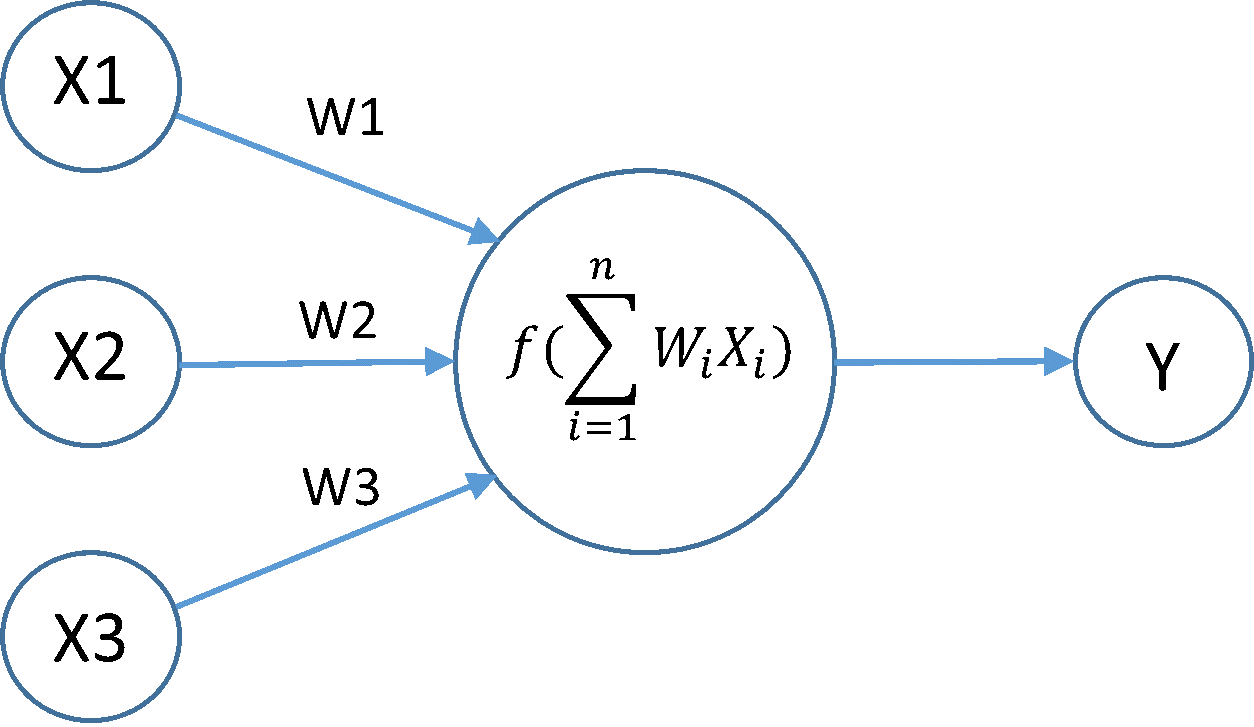
\includegraphics[width=\textwidth]{neuron.png}

Where each of x1,x2,x3x1,x2,x3 are input nodes and w1,w2,w3w1,w2,w3 are weights by which the inputs are multiplied. The summation of the products is passed through an activation function, the value of which is called the output of the neuron. In almost all present day applications, a combination of these neurons is used to make learning models. They may contain several hidden layers with each layer containing several neurons.




\end{document}
